\begin{figure}[H]
\centering
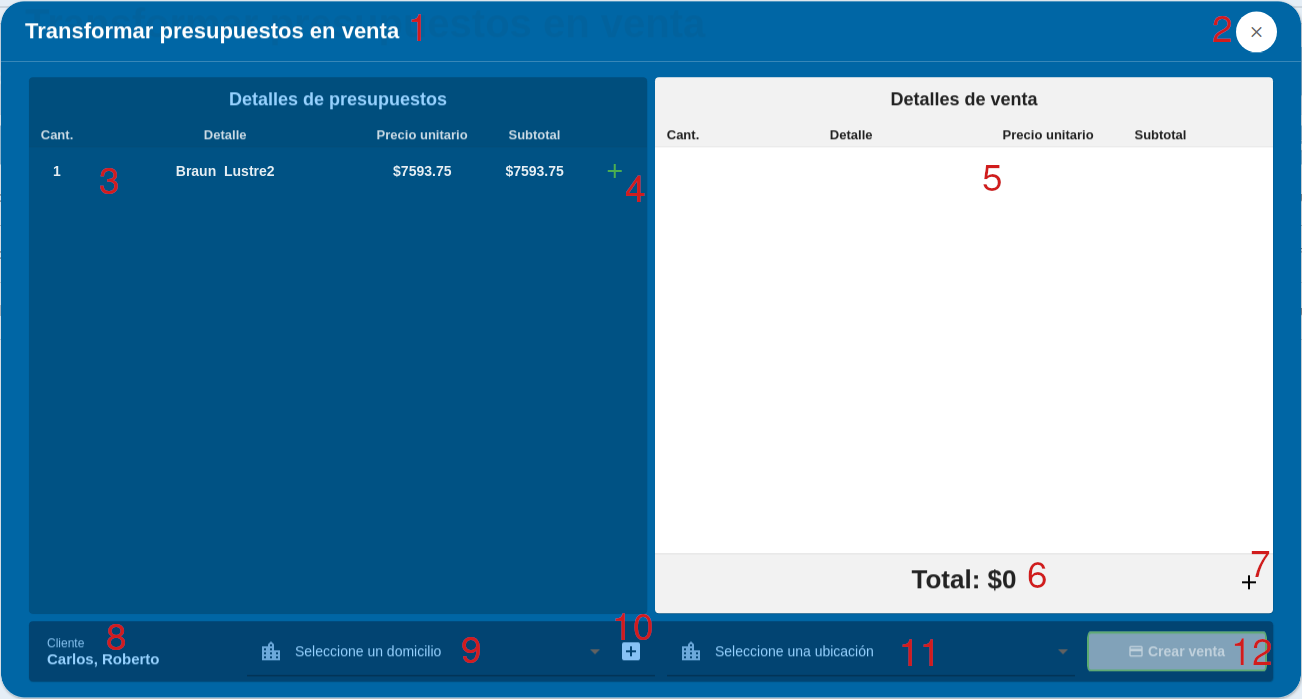
\includegraphics[width=\textwidth,height=\textheight,keepaspectratio]{Escenarios/AD-08-00}
\caption{Escenario - AD-08-00}
\label{fig:AD-08-00}
\end{figure}
Este es el escenario que permite a los usuarios crear una venta a partir de uno más presupuestos. El titulo \textbf{AD-08-01} indica la operación a realizar. Con el botón \textbf{AD-08-02} se podrá cerrar la ventana y volver al escenario \textbf{AD-03-00}.
En la sección \textbf{AD-08-03} se muestra toda la información de los presupuestos seleccionados. El boton \textbf{AD-08-04} permite seleccionar las líneas de presupuestos con las cuales se creará posteriormente la venta. En la sección \textbf{AD-08-05} se mostrará información de las líneas con las cuales se creará la venta, que podrás ser seleccionadas de las sección \textbf{AD-08-03} o bien creadas. En el campo \textbf{AD-08-06} se mostrará el total de la venta a crear. El boton \textbf{AD-08-07} al escenario \textbf{AD-05-00} para crear una nueva linea de venta.
En el campo \textbf{AD-08-08} se muestra el cliente para el cual se creará la venta. En la lista desplegable \textbf{AD-08-09} se mostrarán los domicilios del cliente, de los cuales el usuario deberá elegir uno para la venta. El botón \textbf{AD-08-10} navega al escenario \textbf{AD-31-00} para crear un domicilio para el cliente. La lista desplegable \textbf{AD-08-11} muestra todas las ubicaciones y el usuario seleccionará en la cual se está creando la venta. Un click en el botón \textbf{AD-08-12} creará la venta y navegará al escenario \textbf{AD-09-00}.
\clearpage
